\subsection{Нейронные сети}\label{subsec:neural_network}
%\addcontentsline{toc}{subsection}{Нейронные сети}

\begin{definition}
  Искусственная нейронная сеть (нейронная сеть)~---~математическая модель, а~также её программная реализация, построенная по~принципу организации и функционирования биологических нейронных сетей.
\end{definition}
Это понятие возникло при~изучении процессов, протекающих в~мозге, и при~попытке смоделировать их. После разработки алгоритмов обучения получаемые модели стали использовать в~практических целях: в~задачах прогнозирования, для~распознавания образов, в~задачах управления и др.
Нейронная сеть представляет собой систему соединённых и взаимодействующих между собой простых процессоров (искусственных нейронов).
Каждый процессор подобной сети имеет дело только с~сигналами, которые он получает, и сигналами, которые он периодически посылает другим процессорам. И, тем~не~менее, будучи соединёнными в~достаточно большую сеть с~управляемым взаимодействием, такие по~отдельности простые процессоры вместе способны выполнять сложные задачи.

Нейронные сети не программируются в~привычном смысле этого слова, они обучаются. Возможность обучения~--~одно из~главных преимуществ нейронных сетей перед традиционными алгоритмами. Технически обучение заключается в~нахождении коэффициентов связей между нейронами. В~процессе обучения нейронная сеть способна выявлять сложные зависимости между входными данными и выходными, а~также выполнять обобщение. Это значит, что в~случае успешного обучения сеть сможет вернуть верный результат на~основании данных, которые отсутствовали в~обучающей выборке, а~также неполных и/или «зашумленных», частично искажённых данных.

\begin{figure}[h]
    \centering
    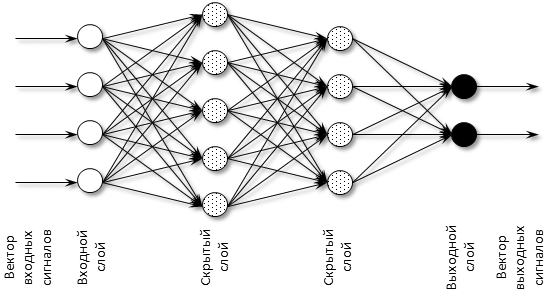
\includegraphics[width=0.8\textwidth]{nn_vizualisation}
    \caption{Полносвязная нейронная сеть.}
    \label{fig:nn}
\end{figure}

Обучение полносвязной\cite[с.\,44]{bib:neural_networks} нейронной сети с~$L$ скрытыми слоями\cite[с.\,43]{bib:neural_networks} происходит в несколько этапов. Для каждого вектора из набора данных выполняются следующие операции:
\begin{enumerate}\label{alg:neural_education}
\item Вектор входных параметров $x_0$ передается на входной слой~$l_0$ нейронной сети.
\item От каждого нейрона входного слоя значения передаются к каждому из $K_1$ нейронов первого скрытого слоя $l_1$ нейронной сети.
\item Каждый нейрон скрытого слоя вычисляет скалярное произведение \newline $y~=~\langle~W_i, x_{i-1}~\rangle$, где $i\in\{1; \dots; L\}$~-~номер текущего слоя, $W_i$~-~вектор весов $i$-го слоя, а $x_{i-1}$~-~вектор значений, полученных с $(i-1)$-го слоя.
\item Вычисляется выходное значение нейрона $x_i = f_{a_i}(y)$, где $f_{a_i}$~-~функция активации\cite[с.\,151]{bib:neural_networks2} $i$-го слоя.
\item Выходное значение $x_i$ передается каждому из $K_{i+1}$ нейронов следющего слоя. Если следующий слой не~является выходным, то~повторяются шаги (3)-(4), иначе полученный вектор выходных значений~$x_{L+1}$ является ответом нейронной сети.
\end{enumerate}
Далее, векторы $x_{L+1}$, полученные для~каждого элемента из~набора данных, сравниваются по~заданной метрике\cite{bib:metrics} $\rho$ с~ответами
и вычислятся значение функции потерь\cite[с.\,65]{bib:neural_networks2} $f_{loss}$. После чего веса $W_i$ для $i\in\{1; \dots; L\}$ пересчитываются по~методу обратного распространения ошибки\cite[с.\,151-184]{bib:neural_networks2} и алгоритм повторяется.

Таким образом, нейронная сеть задается следующими параметрами: количество скрытых слоев $L$, функция активации $f_{a,i}$ и количество нейронов $K_i$ для $i\in\{1; \dots; L\}$, функция потерь $f_{loss}$ и метрика $\rho$.

%\newpage 